\documentclass[12pt]{article}
\usepackage{amsmath}
\usepackage{amssymb}
\usepackage{fancyhdr}
\usepackage{geometry}
\usepackage{hanging}
\usepackage{enumitem}
\usepackage{graphicx}
\usepackage{setspace}
\usepackage{tabularx}
\usepackage{array}
\usepackage{xcolor}
\usepackage{longtable}
%\usepackage{lipsum} %remove later
\doublespacing
%\setlength\parindent{28 pt}
\geometry{letterpaper, margin=1in}

% ++++ Fancy Settings (for header) ++++
\pagestyle{plain}
\fancypagestyle{main}{
	\fancyhf{}
	\lhead{Firewall Configuration}
	\rhead{\leftmark}
	\cfoot{\thepage}
	\renewcommand{\headrulewidth}{0.4pt}
}

% Column widths (tweak the numbers if you want)
\newcommand{\colNum}{0.02\linewidth}
\newcommand{\colSmall}{0.10\linewidth}   % column 1 (1–10)
\newcommand{\colMed}{0.16\linewidth} % columns 2,3,5
\newcommand{\colBig}{0.20\linewidth}   % column 4 (3x colSmall)

% ++++ Begin Doc ++++

\begin{document}

% ++++ Cover Page ++++

\begin{titlepage}
\centering
\vfill

% ++Logo
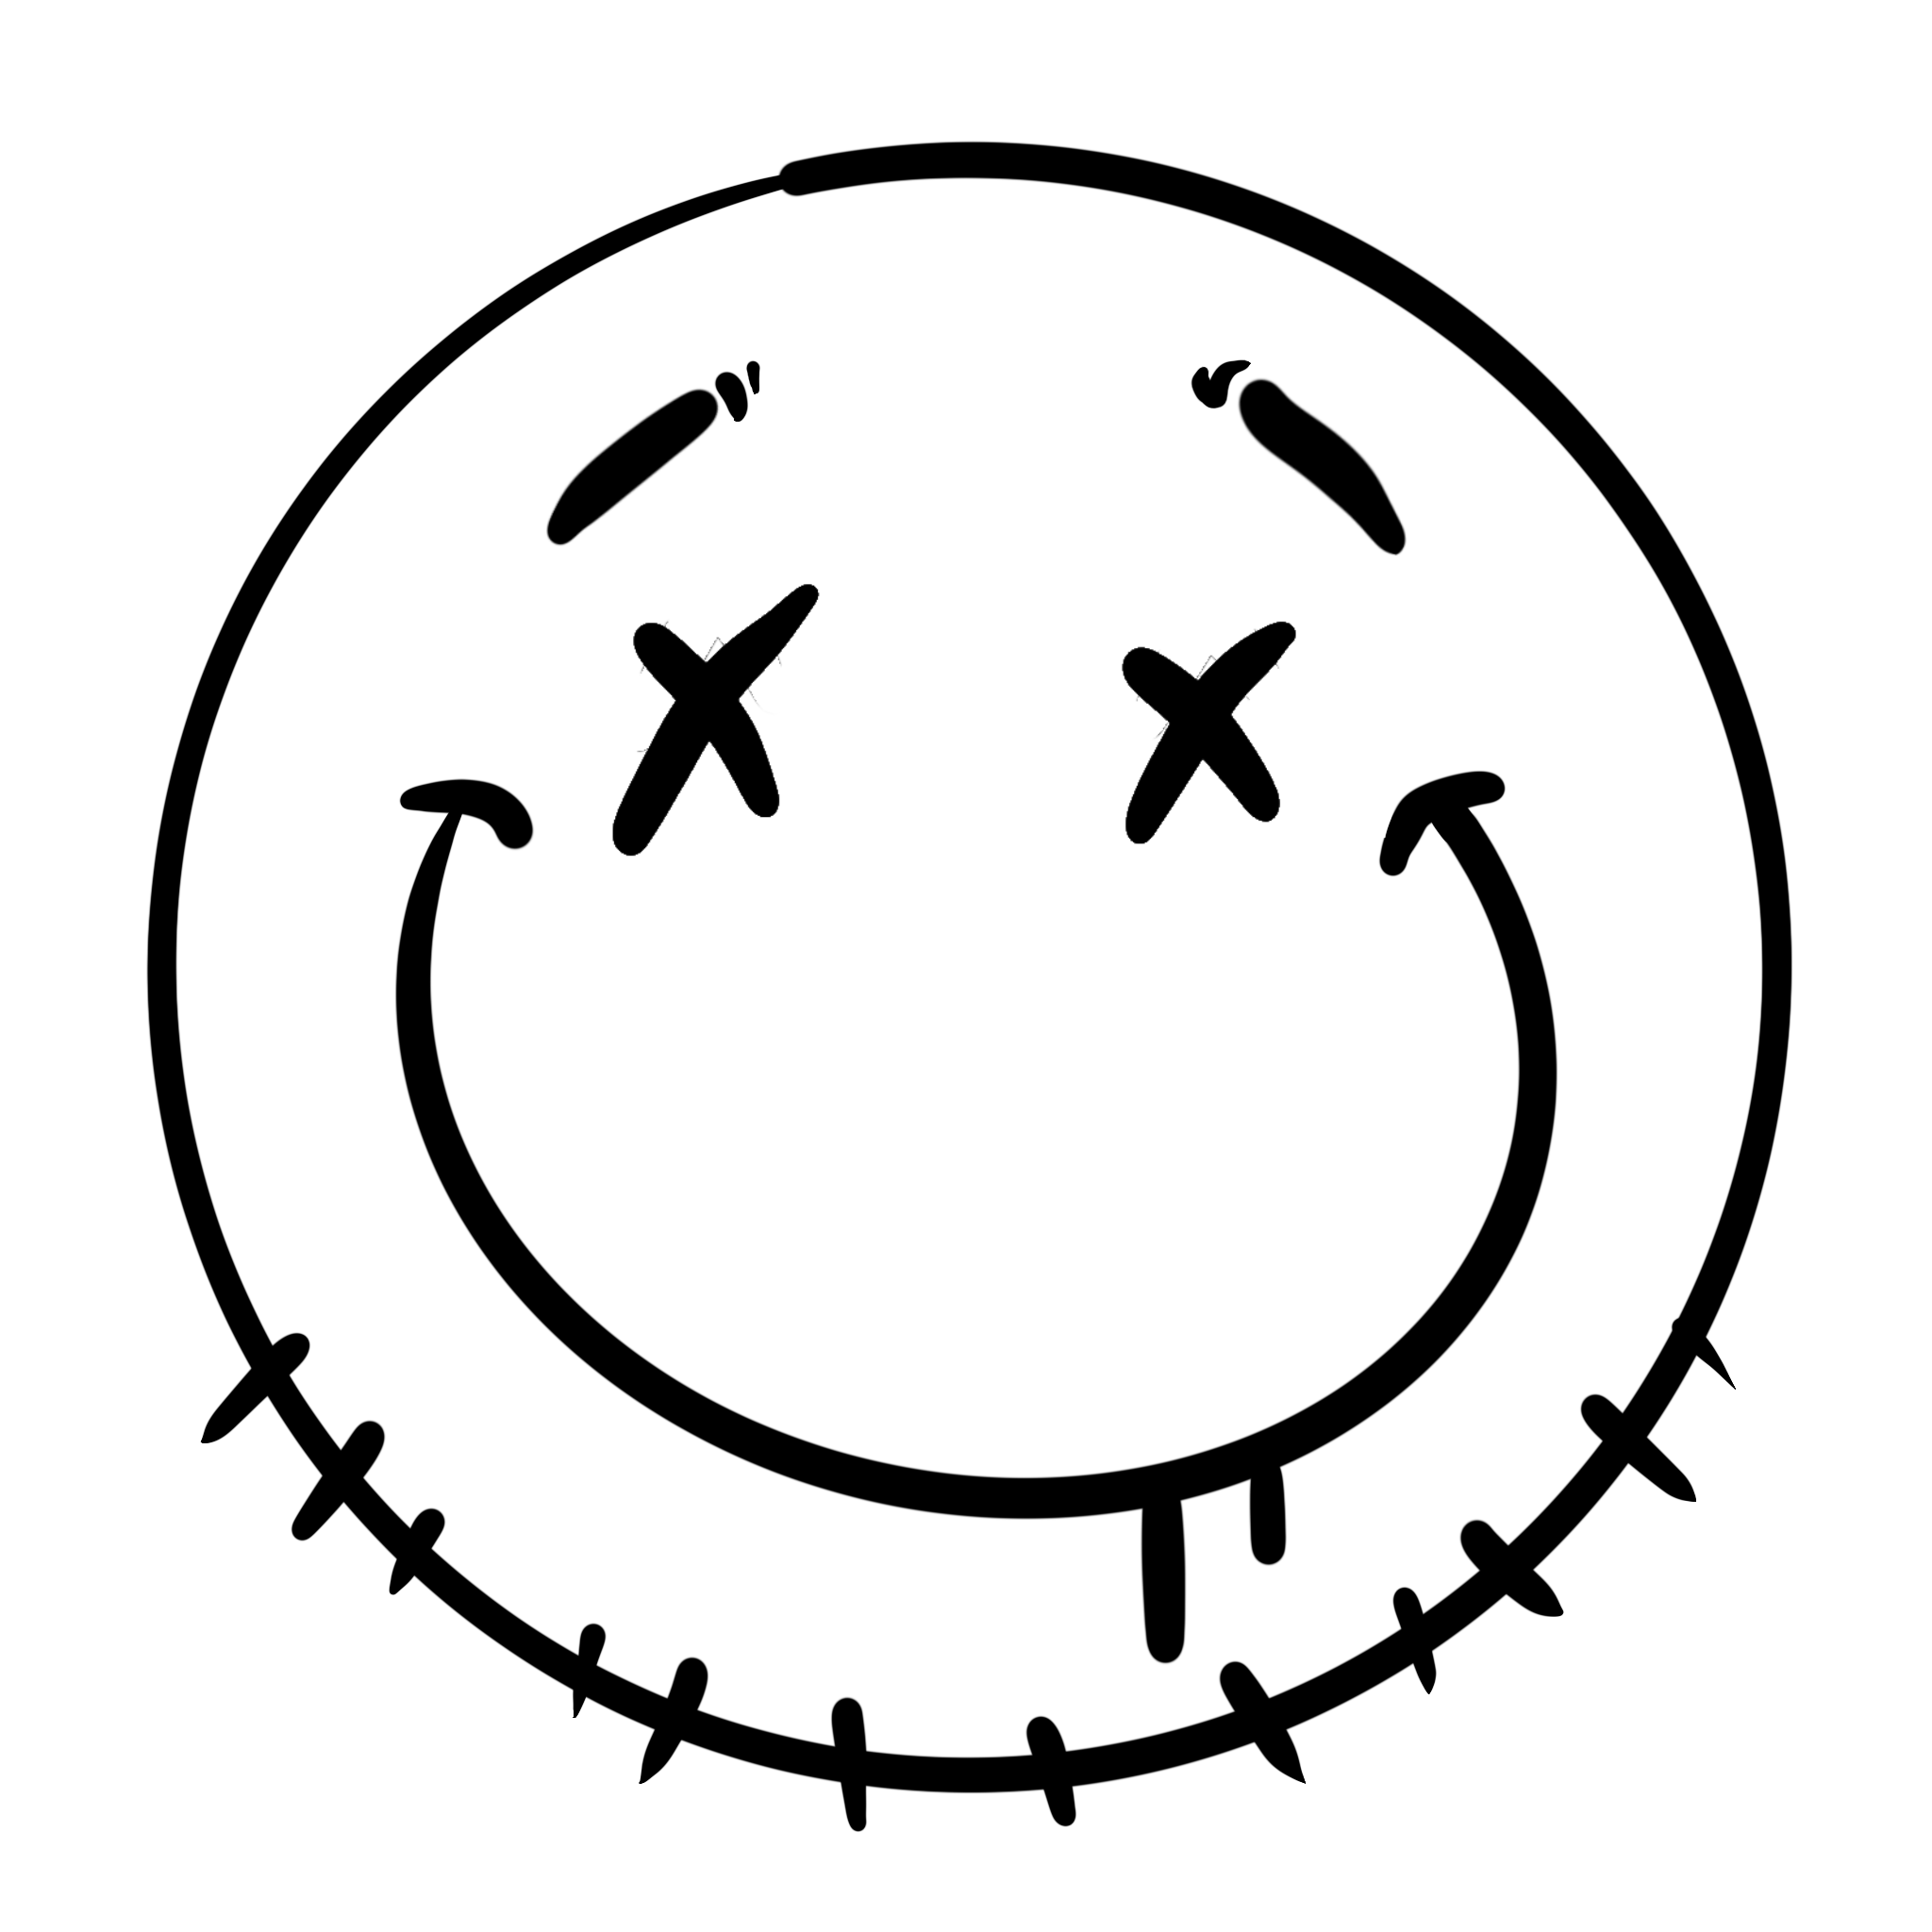
\includegraphics[width=0.35\textwidth]{images/logo.png}

\vspace{1.5cm}

% ++Title
\LARGE{\textbf{Firewall Configuration}}\\
\vspace{0.3cm}
\large{\textbf{Keith Schoen}}\\
\vspace{0.3cm}
\large{\textbf{CSEC 3755-001}}\\
\vspace{0.3cm}
\large{\textbf{Dr. Daniel Pittman}}\\
\vspace{0.3cm}
\large{\textbf{28 April 2026}}\\
\vspace{0.3cm}

\vfill
\end{titlepage}

% ++++ ToC ++++

\pagenumbering{gobble} %hide page numbers for cover and ToC
\tableofcontents
\clearpage

% ++++ Begin Report ++++

\pagenumbering{arabic} %page one starts here
\setcounter{page}{1}
\pagestyle{main} %turn on fancy

% ++++ Part 1 ++++
\section{Current State Analysis}
\subsection{Firewall Rules (iptables)}
INPUT chain - default policy ACCEPT:
\begin{itemize}
	\item Rule 1: ICMP accepted from anywhere
\end{itemize}
FORWARD chain - default policy ACCEPT:
\begin{itemize}
	\item Rule 1: All traffic forwarded eth0 $\rightarrow$ eth1
	\item Rule 2: All traffic forwarded eth1 $\rightarrow$ eth0
\end{itemize}
OUTPUT chain - default policy ACCEPT:
\begin{itemize}
	\item No rules; completely open
\end{itemize}
\subsection{Identified Gaps and Weaknesses}
\begin{enumerate}
	\item \textbf{Default ACCEPT policies} - All three chains accept everything by default. A secure firewall should default to DROP.
	\item \textbf{Unrestricted forwarding} - All traffic passes freely between networks with no port or protocol filtering.
	\item \textbf{No stateful inspection} - No rules tracking established/related connections.
	\item \textbf{Management services exposed on all interfaces} - SSH and Webmin reachable from both the scan network and target network.
	\item \textbf{Webmin on port 1000} - Web-based admin panel is a significant attack surface and should be restricted to a trusted management IP only.
	\item \textbf{IIS 10.0 version disclosure} - Web server advertises its version in HTTP headers, aiding potential attackers in finding known vulnerabilities.
\end{enumerate}
\textbf{Service That Should Be Restricted Between Zones}
\begin{itemize}
	\item \textbf{SSH (port 22)} - Should only be reachable from the scan/management network, not from the target network.
	\item \textbf{Webmin (port 10000)} - Should be restricted to a single trusted IP, not exposed to any network broadly.
	\item \textbf{All forwarded traffic} - Should be whitelisted by specific port/protocol rather than allowing everything through.
\end{itemize}
\section{Proposed Ruleset (By Section)}
\textbf{Chain 1: INPUT (traffic destined for the router itself)}\\
\ \\
\noindent \textbf{Default policy:} \texttt{DROP}
{\singlespacing
	\begin{longtable}{
 		|| >{\centering\arraybackslash}p{\colNum}
  		| >{\raggedright\arraybackslash}p{\colMed}
  		| >{\raggedright\arraybackslash}p{\colSmall}
  		| >{\raggedright\arraybackslash}p{\colMed}
  		| >{\raggedright\arraybackslash}p{\colSmall} 
		| >{\raggedright\arraybackslash}p{\colSmall}
  		| >{\raggedright\arraybackslash}p{\colMed}||}
		\hline
		\textbf{\#} & \textbf{Name} & \textbf{Source} & \textbf{Destination} & \textbf{Port} & \small{\textbf{Action}}& \textbf{Justification} \\
		\hline\hline
		\endhead
		\hline
  	    	 1 & Allow loopback & 127.0.0.1 & 127.0.0.1 & any & Allow  & Required for local system processes \\
		\hline
  	    	 2 & Allow SSH management & eth0 & Router  & 22 & Allow & Administrators need remote access from scan-net side only \\
		\hline
  	    	 3 & Allow ICMP & eth0 & Router  & ICMP & Allow  & Network diagnostics and connectivity verification \\
	    \hline
  	    	 4 & Allow established/ relate & Any & Router & Any & Allow & Stateful tracking for connections initiated by the router \\
		\hline
  	    	 5 & Default deny INPUT & Any & Router  & Any & Drop  & Reject all traffic not explicitly permitted \\
		\hline
	\end{longtable}
}
\noindent\textbf{Chain 2: FORWARD (traffic passing through the router between zones)}\\
\ \\
\noindent \textbf{Default policy:} \texttt{DROP}
{\singlespacing
	\begin{longtable}{
 		|| >{\centering\arraybackslash}p{\colNum}
  		| >{\raggedright\arraybackslash}p{\colMed}
  		| >{\raggedright\arraybackslash}p{\colSmall}
  		| >{\raggedright\arraybackslash}p{\colMed}
  		| >{\raggedright\arraybackslash}p{\colSmall} 
		| >{\raggedright\arraybackslash}p{\colSmall}
  		| >{\raggedright\arraybackslash}p{\colMed}||}
		\hline
		\textbf{\#} & \textbf{Name} & \textbf{Source} & \textbf{Destination} & \textbf{Port} & \small{\textbf{Action}}& \textbf{Justification} \\
		\hline\hline
		\endhead
		\hline
  	    	 1 & Allow Established/ Related & Any & Any & Any & Allow & Stateful tracking for all forwarded connections \\
		\hline
  	    	 2 & Allow HTTP to taget-net & eth0 & eth1 & 80 & Allow  & Permits web access to IIS and patient portal services \\
		\hline
  	    	 3 & Allow HTTPS to target-net & eth0 & eth1 & 443 & Allow  & Encrypted web traffic to target services \\
	    \hline
  	    	 4 & Allow SSH to target-net & eth0 & eth1 & 22 & Allow & Administrative access to connected machines \\
		\hline
  	    	 5 & Allow ICMP to target-net & eth0 & eth1 & ICMP & Allow & Network diagnostics and host discovery \\
		\hline
		  	 6 & Block target-net outbound & eth1 & eth0 & Any & Block & Compromised internal machines cannot initiate connections outbound \\
		\hline
  	    	 7 & Default deny \texttt{FORWARD} & Any & Any & Any & Drop & No other cross-zone traffic is business justified \\
		\hline
	\end{longtable}
}
\newpage
\noindent\textbf{Chain 3: OUTPUT (traffic originating from the router itself)}\\
\ \\
\noindent \textbf{Default policy:} \texttt{ACCEPT}
{\singlespacing
	\begin{longtable}{
 		|| >{\centering\arraybackslash}p{\colNum}
  		| >{\raggedright\arraybackslash}p{\colMed}
  		| >{\raggedright\arraybackslash}p{\colSmall}
  		| >{\raggedright\arraybackslash}p{\colMed}
  		| >{\raggedright\arraybackslash}p{\colSmall} 
		| >{\raggedright\arraybackslash}p{\colSmall}
  		| >{\raggedright\arraybackslash}p{\colMed}||}
		\hline
		\textbf{\#} & \textbf{Name} & \textbf{Source} & \textbf{Destination} & \textbf{Port} & \small{\textbf{Action}}& \textbf{Justification} \\
		\hline\hline
		\endhead
		\hline
  	    	 1 & Allow all router output & Router  & Any & Any  & Allow & Router requires free communication for DNS, NTP, and management functions \\
		\hline
	\end{longtable}
}
\newpage
\section{Testing Results}
To test the newly implemented firewall rules, the first step was to run a nmap scan from my Kali machine to see what is now visible through the firewall now that the rules have been updated. \\
\begin{itemize}
	\item \textbf{What was blocked:} RDP (3389), SMB (445/139), MySQL (3306), FTP (21), SMTP (25), RPC (135), and WinRM (5985)
	\item \textbf{What still flows:} HTTP (80), and SSH (22) on both Ubuntu and Windows, and SSH on the router
\end{itemize}

\includegraphics[width=0.50\textwidth]{images/nmap-before/1.png} \\ 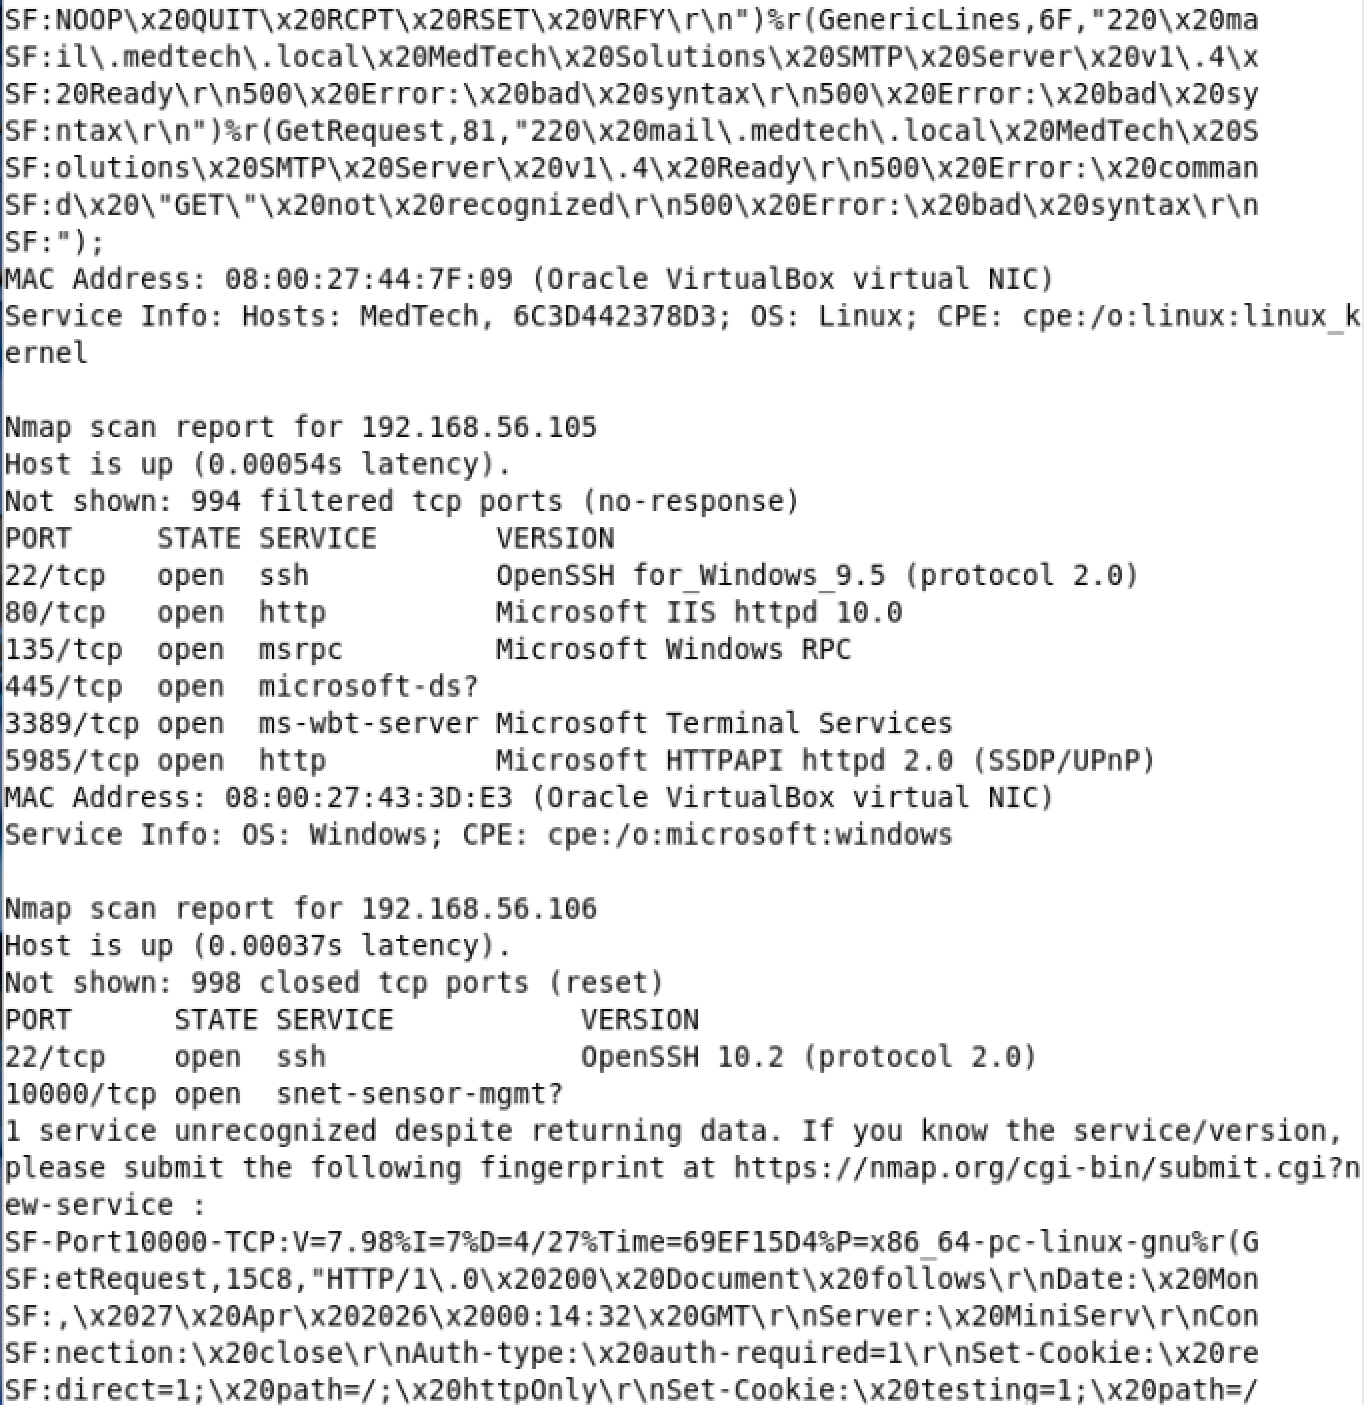
\includegraphics[width=0.50\textwidth]{images/nmap-before/2.png} \\ 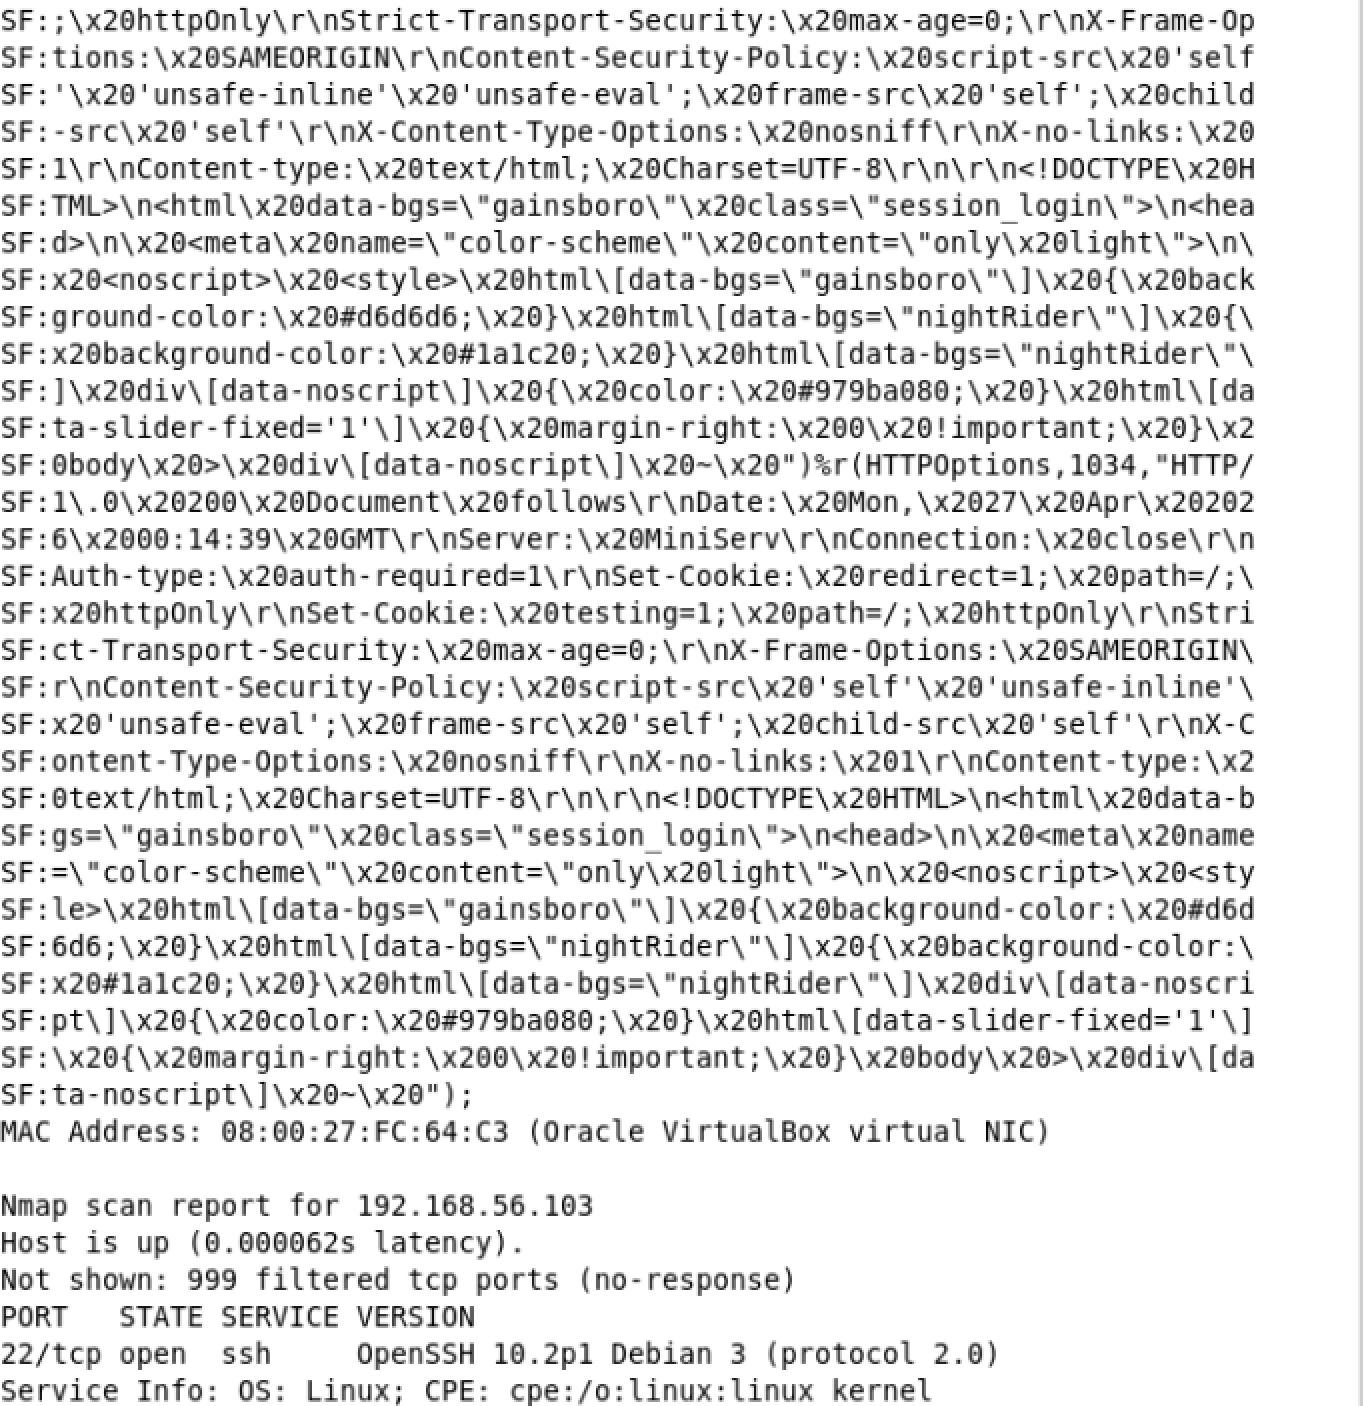
\includegraphics[width=0.50\textwidth]{images/nmap-before/3.png} \\ 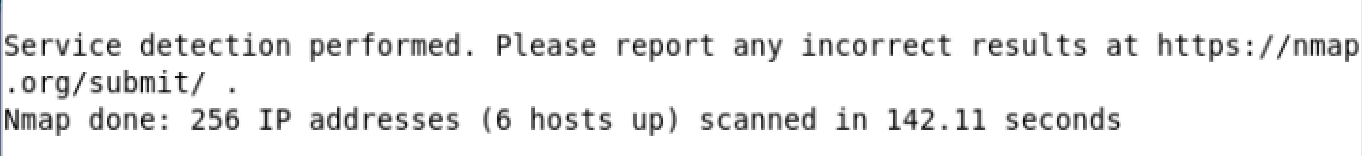
\includegraphics[width=0.50\textwidth]{images/nmap-before/4.png} \\ \textit{Figure 01-04: Result of nmap scan of subnet before firewall rules were implemented}\\
\ \\
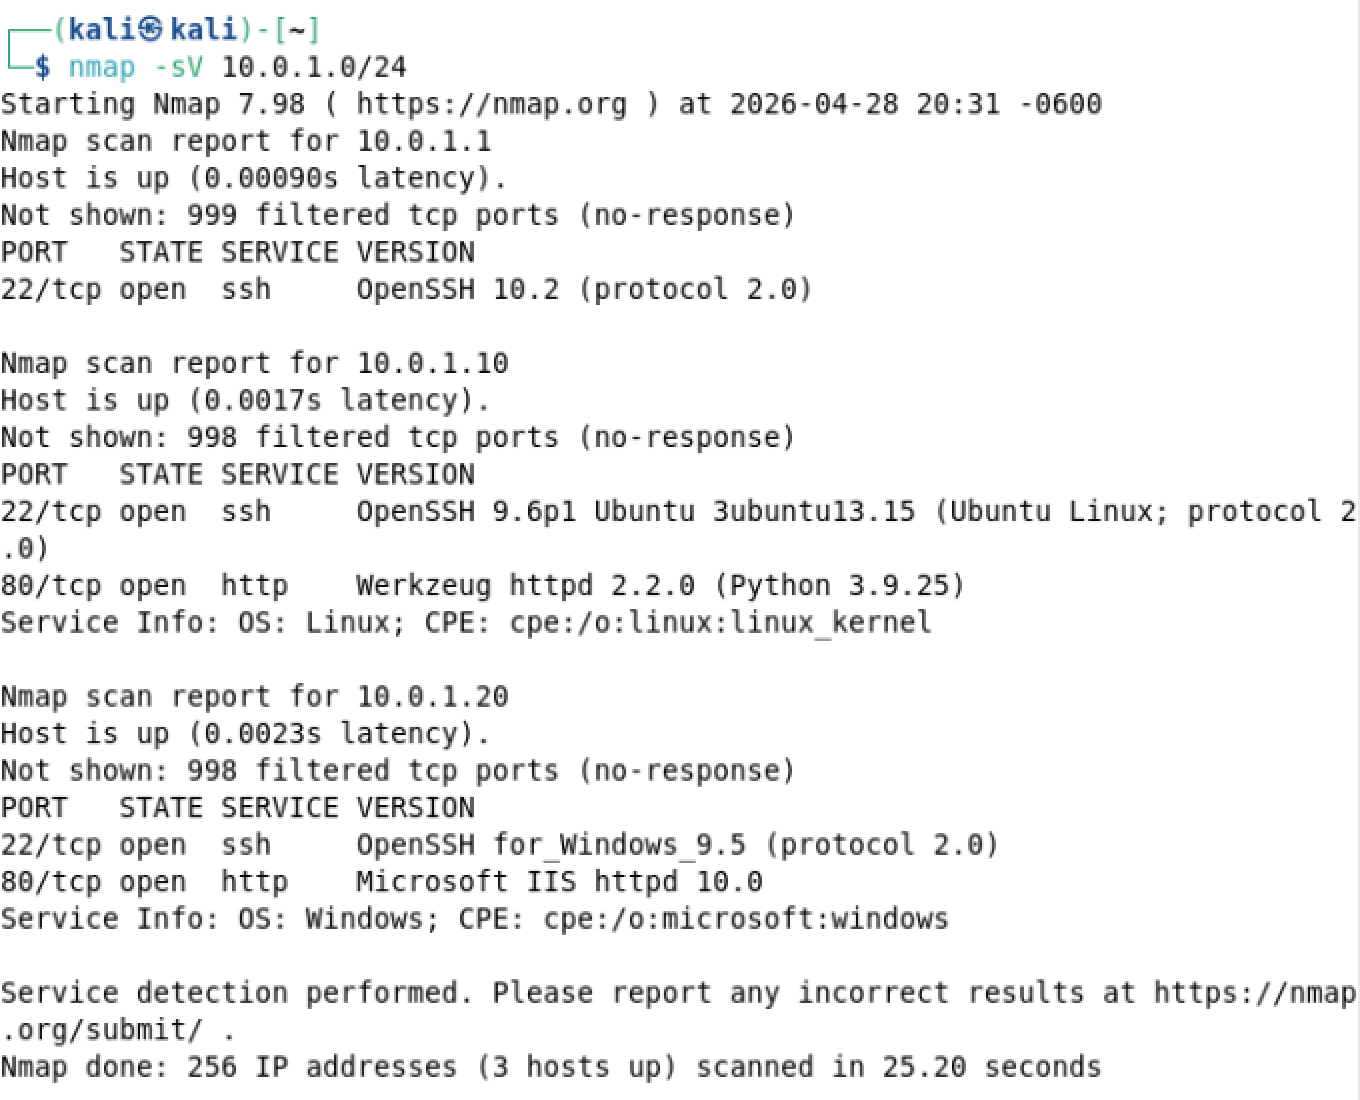
\includegraphics[width=0.50\textwidth]{images/nmap-after/1.png} \\ \textit{Figure 05: Result of nmap scan after rules were implemented.}

\vfill
\textit{++report written with (minimal) help from Claude (Sonnet 4.6)++}
\end{document}

% +++++++++ Helpful stuff +++++++++++
%
% +++ Using Minipages +++
% \begin{minipage}[t]{\linewidth}
% \includegraphics[width=0.50\textwidth]{*Image file}\\
% \textit{*Image subtitle}
% \end{minipage}
% \end{enumerate}
%


% +++ Fixed width table +++
%\begin{tabularx}{1.0\textwidth}{
%	|| >{\raggedright\arraybackslash}X
%	|  >{\raggedright\arraybackslash}X
%	|  >{\raggedright\arraybackslash}X
%	|  >{\raggedright\arraybackslash}X || }
%	\hline
%	\textbf{x} & \textbf{x} & \textbf{x} & \textbf{x} \\
%	\hline \hline
%	x $ x $ x & x & x & x  \\
%	\hline
%	x $ x $ x & x & x & x \\
%	\hline
%	x $ x $ x & x & x & x \\
%	\hline
%	x $ x $ x & x &  x  & x \\
%	\hline
%\end{tabularx}
%

% +++ For tables that take multiple pages +++
%{\singlespacing
%	\begin{longtable}{
% 		|| >{\centering\arraybackslash}p{\colNum}
%  		| >{\raggedright\arraybackslash}p{\colSmall}
%  		| >{\raggedright\arraybackslash}p{\colSmall}
%  		| >{\raggedright\arraybackslash}p{\colBig}
%  		| >{\raggedright\arraybackslash}p{\colSmall} ||}
%		\hline
%		\textbf{x} & \textbf{x} & \textbf{x} & \textbf{x} & \textbf{x} \\
%		\hline\hline
%		\endhead
%		\hline
%  	    	 x & x & x & x  & x \\
%		\hline
%	\end{longtable}
%}












